\section{Klassische statistische Mechanik}
\subsection{mikroskopische Bedeutung von Druck und Temperatur}
\begin{tabular}{p{4cm} p{15cm}}
$k_B$	& $k_B = 1.3807 \cdot 10^{-23} J/K$\\
Geschwindigkeit	& \begin{tabular}[t]{l}
               	  $\langle v_x^2 \rangle = \frac{1}{N} \sum_{i=1}^N v_{xi}^2$\\
		  Bewegung isotrop: $\langle v_x^2 \rangle = \langle v_y^2 \rangle = \langle v_z^2 \rangle = \frac{1}{3} \langle v^2 \rangle$\\
		  $\langle v^2 \rangle = \langle v_x^2 \rangle + \langle v_y^2 \rangle + \langle v_z^2 \rangle$
               	  \end{tabular}\\
Druck	& \begin{tabular}[t]{l}
     	   $p = \frac{F}{A}$\\
	   $p = \frac{1}{3} \rho \langle v^2 \rangle$\\
	   $p = \frac{2}{3}\frac{N}{V} \left( \frac{1}{2}m \langle v^2 \rangle \right) = \frac{2}{3} \frac{N}{V} \langle E_{kin} \rangle \Leftrightarrow pV = \frac{2}{3}N\langle E_{kin} \rangle (\ast)$
     	  \end{tabular}\\
Dichte	& $\rho = \frac{mN}{V}$\\
Zustandsgleichung ideales Gas	& $pV = Nk_B T$\\
Temperatur: �quipartitionsgesetz	& Mit der Zustandsgleichung ergibt sich aus $(\ast) \langle E_{kin} \rangle = \frac{3}{2}k_BT$. Isotropie vorausgesetzt, ist die innere Energie also pro Freiheitsgrad $\langle E_{kin,j} \rangle = \frac{1}{2} k_BT\quad j = x,y,z$.\\
			& $\langle E_{kin} = U \rangle = \frac{f}{2} k_BT\quad $ f = \# Freiheitsgrade $\cdot$ \# Molek�le $\quad U:$ Innere Energie\\
G�ltigkeit �PG		& Das �quipartitionsgesetz ist bei tiefen Temperaturen nicht mehr g�ltig, wegen der Quantisierung der Energiezust�nde.\\
Freiheitsgrade		& \begin{tabular}[t]{ll}
			    \multicolumn{2}{l}{F�r zweiatomige Molek�le gelten bspw. folgende Freiheitsgrade}\\
			    Translation des Schwerpunkts	& $f=3$\\
			    Rotation				& $f=2$\\
			    Vibration				& $f=2$
			  \end{tabular}
\end{tabular}\\

\subsection{Ensembles}
\begin{tabular}{p{4cm} p{15cm}}
$n_i$	& Anz. Teilchen\\
$P$	& WSK, dass ein System in einer bestimmten Zustandskonfiguration ist.\\
$g_i$	& WSK, ein Teilchen in einem bestimmtem Zustand zu finden.\\
Thermodyn. Glgw. (TG)	& dP = 0\\
\end{tabular}
\subsubsection{Kanonisches Ensemble}
\begin{tabular}{p{4cm} p{15cm}}
Konstanten	& $N,V,T$\\
Fluktuationen	& $E$\\
		& $N = \sum_i n_i$\\
$g_i$ (unter TG)	& $\boxed{g_i = \frac{1}{Z(N,V,T)} e^{-\beta E_i}}$\\
Kanonische Zustandssumme	& $\boxed{Z(N,V,T) = \sum_i g_i e^{-\beta E_i}}\quad \beta = \frac{1}{k_BT}$\\
Energie				& $\boxed{\langle E \rangle = \sum_i g_i E_i} = - \left( \frac{\partial \ln Z(N,V,T)}{\partial \beta} \right)_{N,V}$\\
Druck			& $\langle p \rangle = \frac{1}{\beta} \left( \frac{\partial \ln Z(N,V,T)}{\partial V} \right)_{N,\beta}\quad \Delta E_i = -p_i\Delta V$\\
Entropie		& $S = -k_B \sum_i g_i \ln g_i$\\
Zustandssumme ideales Gas	& \begin{tabular}[t]{l}
				      $Z_{id} = \sum_i g_i e^{-E_i/k_BT} = \int_0^{\infty} D_3(E) e^{-E/k_BT} dE$\\
				      $\quad D_3(E) = \frac{L^3}{2\pi^2}\left( \frac{2m}{\hbar^2} \right)^{\frac{3}{2}} \sqrt{E} dE$\\
				      $Z_{id} = \frac{V(2\pi mk_BT)^{3/2}}{h^3} = V\left( \frac{m}{2\beta\pi\hbar^2} \right)^{\tfrac{3}{2}}$
				  \end{tabular}\\
Anzahl Molek�le w.r.t. Energie	& $dn = \frac{N}{Z}e^{-E/k_BT}D(E) dE$\\
				& 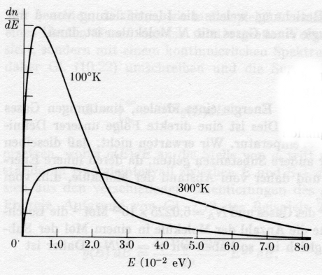
\includegraphics[width = 7cm]{ph_statmech_dndE.png} 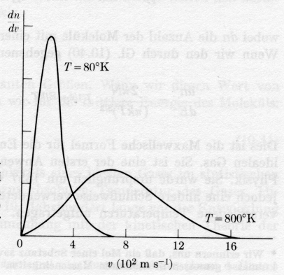
\includegraphics[width = 7cm]{ph_statmech_dndv.png}\\
\end{tabular}
\subsubsection{Maxwell-Boltzmann-Verteilung}
\begin{tabular}{p{4cm} p{15cm}}
Zustandssumme		& $Z(N,V,T) = \frac{1}{N!}[z(V,T)]^N$\\
Ideal Gas		& \\
Avg. size of velocity	& $\langle v \rangle = \sqrt{ \frac{8k_BT}{m\pi} }$\\
Root mean square	& $\langle v^2 \rangle^\frac{1}{2} = \sqrt{ \frac{3k_BT}{m} }$\\
most probable speed	& $v_{mp} = \sqrt{ \frac{2k_BT}{m}}$\\
Avg. kinetic energy	& $\langle E \rangle = N \frac{3}{2} k_BT$\\
Heat capacity		& $\frac{dE}{dT} = \frac{3}{2} Nk_B$\\
Free energy		& $F = -Nk_BT \left( \frac{3}{2} \ln \left(\frac{2\pi mk_BT}{h^2} \right) - \ln \left( \frac{N}{V} \right) + 1 \right)$\\
Entropy			& $S = Nk_B \left( \frac{3}{2} \ln \left(\frac{2\pi mk_BT}{\hbar^2} \right) - \ln \left( \frac{N}{V} \right) + \frac{5}{2} \right)$
\end{tabular}
\subsection{Fermi-Dirac, Bose-Einstein partition functions}
\begin{tabular}{p{4cm} >{$}p{16cm}<{$}}
System			& \text{
			    \begin{tabular}{l}
			      Volume: $V$\\
			      Number of particles: $N$\\
			      Energy levels: $E_j$\\
			      1-particle energy levels: $\epsilon_k$\\
			      Number of particles in a quantum state $\Psi_k: m_k$\\
			    \end{tabular}
			  }\\
			& E_j = \sum_k m_k\epsilon_k; N = \sum_k m_k\\
Grand-canonical partition function	& Z(\mu,V,T) = \sum_{N=0}^{\infty}\sum_j e^{-\beta (E_j-\mu N)} = ... = \prod_k\sum_{m_k} \left( e^{-\beta(\epsilon_k-\mu)}\right)^{m_k}\\
Fermi-Dirac partition function	& m_k = 0 \vee 1 \Rightarrow Z_{FD} (\mu,V,T) = \prod_k \left[ 1+e^{-\beta(\epsilon_k-\mu)} \right]\\
Bose-Einstein partition function	& m_k = 0,1,2,... \Rightarrow Z_{BE} (\mu,V,T) = \prod_k \left[ 1-e^{-\beta(\epsilon_k-\mu)} \right]^{-1}\\
Combined partition function		& Z_{FD/BE}(\mu,V,T) = \prod_k \left[ 1\pm e^{-\beta(\epsilon_k-\mu)} \right]^{\pm 1}
\end{tabular}\\
\subsection{Fermi-Dirac Statistics}
\begin{tabular}{p{4cm} >{$}p{16cm}<{$}}
Avg. Number of particles	& \langle N \rangle = \frac{1}{\beta} \left( \frac{\partial \ln Z_{FD}(\mu,V,T) }{\partial \mu} \right)_{V,T} = ... = \sum_k \left(e^{+\beta(\epsilon_k-\mu)} + 1 \right)^{-1} = \sum_k \langle m_k \rangle\\
$\langle m_k \rangle$		& \langle m_k \rangle = e^{-\beta(\epsilon_k-\mu)}\quad \langle m_k \rangle << 1 \text{ (Boltzmann Limit) }\\
Avg. Energy			& \langle E \rangle = \sum_k \langle m_k \rangle \epsilon_k = \sum_k \frac{\epsilon_k}{e^{+\beta(\epsilon_k-\mu)} + 1}\\
Pressure			& pV = k_BT\ln Z_{FD}(\mu,V,T) = k_BT \sum_k \ln \left( 1 + e^{-(\epsilon_k-\mu)/k_BT} \right)
\end{tabular}
\subsection{Bose-Einstein Statistics}
\begin{tabular}{p{4cm} >{$}p{16cm}<{$}}
Avg. Number of particles	& \langle N \rangle = \frac{1}{\beta} \left( \frac{\partial \ln Z_{BE}(\mu,V,T) }{\partial \mu} \right)_{V,T} = ... = \sum_k \left(e^{+\beta(\epsilon_k-\mu)} - 1 \right)^{-1} = \sum_k \langle m_k \rangle\\
$\langle m_k \rangle$		& \langle m_k \rangle = e^{-\beta(\epsilon_k-\mu)}\\
Avg. Energy			& \langle E \rangle = \sum_k \langle m_k \rangle \epsilon_k = \sum_k \frac{\epsilon_k}{e^{+\beta(\epsilon_k-\mu)} - 1}\\
Pressure			& pV = k_BT\ln Z_{BE}(\mu,V,T) = -k_BT \sum_k \ln \left( 1 - e^{-(\epsilon_k-\mu)/k_BT} \right)
\end{tabular}

